\chapter{Introduction}
\label{section:intro}
Next Generation Sequencing technology has been advancing rapidly with higher sequencing power at lower costs. At the present time, expression profiling by high-throughput technology or RNA sequencing (RNA-seq) can unmask the identities of most RNA species \cite{Yongjun2012}. RNA-seq can provide the entire transcriptome of a sample in a single analysis, in a single day \cite{Grada}; with traditional methodologies, such as Sanger sequencing, this process would take minimum 4 to 6 weeks with a fully automated large-scale facility \cite{Lei2008}. Moreover, RNA-seq employs deep-sequencing technology revealing the location of transcription variations to a single-base resolution \cite{Keren2019}.

The transcriptome is the entire set of transcripts that a cell has in quantitative and qualitative manner in a period of development or condition. The importance of the transcriptome understanding relapses in the correct interpretation of functional elements of the genome which leads to the comprehension of the diseases’ development \cite{Wang, Costa}. The functionality of the transcriptome is of crucial importance: the transcripts synthesize fit or unfit proteins or RNA molecules with correct or incorrect regulatory roles \cite{Keren}.

Since RNA-seq is the first sequencing-based method which can survey the whole transcriptome in a quantitative manner and with high performance, this technique has been applied in different applications. For example, mapping gene and exon boundaries, examining splicing diversity, discovery of new transcribed regions, determining gene expression, detect different isoforms, cell gene expression signature, among others \cite{Byron, Conesa2016, Costa, Katz, Michael2014, newman15, Wang}.

The process of RNA-seq consists of few steps. Initially, a population or sample of long RNA is converted to a library of complementary DNA (cDNA) fragments through RNA or DNA fragmentation. After, sequencing adaptors are added to one or both sides of each fragment. Then, short sequences are obtained from each RNA fragment using high-throughput technology. The resulting sequence reads are aligned to a reference genome or transcriptome, or assembled de novo to generate a genome-scale transcription map which is qualitative and quantitative for each gene \cite{Wang}.

In this investigation, 14 databases were downloaded from mainly the NCBI Gene Expression Omnibus (GEO) public repository \cite{GEO} and other public studies. These databases come from RNA-seq studies of human brain samples with one of the three neurodegenerative diseases (NDs). After normalization of each dataset, the data derived from the same condition and tissue were coupled into a single integrated set. The later sets were interrogated with varied algorithms in order to find relevant covariates, differentially expressed genes, molecular subtypes of the diseases, enriched pathways, proportion of immune and brain cells, variation in copy number of chromosome segments and repurposed drugs for treatment. The results of all the queries were incorporated in order to give a biological answer as a whole.

\section{Motivation}
Diverse consortia have generated many copious RNA-seq studies focusing on different types of cancer, such as The Cancer Genome Atlas (TCGA) and the Genotype-Tissue Expression (GTEx) programs, leaving other complex diseases, like NDs, to be studied only by isolated groups. Thus, this creates an opportunity to gather public RNA-seq data of NDs in human tissue from isolated research groups and study them as an entirety. Additionally, by leveraging differential gene expression (DGE) analysis, a correlation between the results and the clinical information from the respective studies can be estimated, as well as to find molecular subtypes of the diseases and suggest possible treatment with repurposed drugs. Since RNA-seq has various advantages over common sequencing technology employed today, for example microarrays, this technique will undoubtedly be the first option for researchers in the near future. Hence, it is consequential to define an optimal and complete pipeline for RNA-seq data.

\section{Problem Statement and Context}
Considering this research addresses RNA-seq public datasets from human brain samples with one of three different NDs, some context is given. NDs result from the gradual and progressive loss of neural cells; this loss leads to a nervous system dysfunction. Although, the pathogenesis of these diseases is complex and remains mostly unknown, transcriptomic studies in animal and cell line models suggest that the primary cause are messenger RNA (mRNA) molecules. However, obtaining post-mortem brain tissue samples with undamaged RNA content is considerably difficult \cite{Costa}.

Alzheimer's disease (AD), Parkinson’s disease (PD) and Huntington’s disease (HD) are the NDs subject to analysis in this research. Briefly, AD is a type of dementia that causes loss of memory and other cognitive abilities that interfere with daily life; in its early years the memory loss is mild, but on latest ages the individual loses the ability to respond to their environment. In 2016, 47 million people were affected with AD at the point of dementia; it is expected to reach 131 million people by 2050 due to the rise of life expectancy \cite{WAR}. PD is a chronic, progressive disease starting with a barely noticeable tremor and as it develops the tremor increases, muscles become rigid and automatic movements are lost. The prevalence of PD increases with age and the statistics are: 1087 per 100,000 between 70 to 79 years old; and 1903 per 100,000 in older than 80 years old \cite{Tamara2014}. HD is an inherited neurological illness which causes involuntary movements (chorea), severe emotional disturbances and cognitive decline (dementia). The estimated prevalence of HD is 2.71 per 100,000 worldwide; it is considered as a rare disease \cite{PringsheimHD}. AD, PD and HD are very complex, the patients have an appalling quality of life, they are fatal, and have no cure.

Since the transcriptome is a snapshot of a given condition, biomarkers and expression patterns can be proposed by detecting, analyzing, and comparing the results with the clinical data of the collected samples. Although the population affected by these three NDs is increasing, gathering profuse public data from brain human samples of expression profiling by high-throughput technology is complicated. RNA-seq is at a maturing stage and researchers are starting to move to this technology. Another encountered obstacle in this research is that it exists a high availability of programs for RNA-seq analysis and there is a lack of consensus of best practices and standards for validation of RNA-seq pipelines \cite{Byron}. Hence, data which is generated by different algorithms may present distinct normalization methods (TPM, RPKM, FPKM, number of reads) which thwarts the integration of assorted datasets.

Nowadays, there are several distinct algorithms and tools to carry out distinct types of analysis in RNA data. However, a pipeline to perform a complete analysis of RNA data of a heterogeneous cohort, including DGE, pathway enrichment, immune and brain cell abundance, molecular subtypes, and drug repurposing has not been designed yet. Moreover, these NDs have been investigated separately and no studies have searched for common alterations in these diseases using RNA-seq expression data.


\section{Research Question}
In this research, the following hypothesis is assessed: By formulating an optimal combination of the existing algorithms of transcriptomic analysis on public datasets, common and unique mechanisms of these NDs can be ascertained. Also, the generated knowledge will be corroborated with other genome studies, such as Genome-Wide Association Studies (GWAS) repositories. Moreover, the following questions are intended to be answered.

\begin{itemize}
\item Is it possible to identify novel alterations of NDs with RNA-seq expression data by combining distinct public databases?
\item Can an optimal combination of already known algorithms for RNA-seq expression data for NDs be generated?
\item Does the results obtained from the proposed pipeline return information that has already been presented in other studies or databases?  
\item Can the results given by public RNA-seq expression data be verified with other genome studies?
\item Can repurposed drugs for NDs treatment be suggested by computing disease gene expression signatures?
\item Can molecular subtypes for each ND be determined by clustering the processed expression data of conditions with sufficient number of samples?
\item Does copy number variation analysis be leveraged on RNA data, as an alternative to DNA data, in order to identify significant changes in case vs control samples?
\item Can relevant enriched pathways be distinguished between the NDs and tissues by computing a DGE analysis?
\end{itemize}

\section{Solution Overview}
In order to solve the mentioned problem, first, public RNA-seq expression data will be gathered from GEO platform and other public studies. Then, datasets with the same condition and tissue source will be merged to form the integrated sets; this allows to investigate alterations on a larger number of samples. After normalization and selection of core samples, the DGE analysis will be carried out. Subsequently, several analyses will be performed: alternative copy number variation, gene set enrichment analysis (GSEA), reverse gene expression score analysis for drug repurposing, immune and brain cell composition, and possible subtype identification. The results will be compared to those presented on genome studies, like GWAS (see Fig. \ref{fig:solution-overview}). In the end, these complete set of results are going to be analyzed as a whole to find common and unique mechanisms of each disease.

\begin{figure}[h]
    \centerline{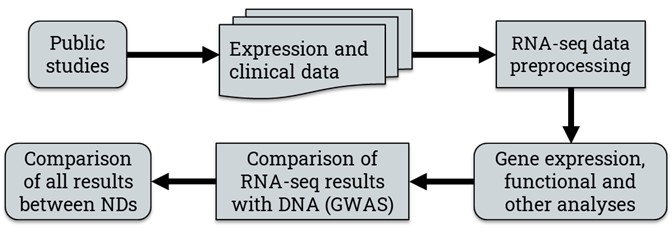
\includegraphics[width = 10cm]{Figures/overview.jpg}}
\caption{Overview of the solution.}
\label{fig:solution-overview}
\end{figure}

The general objective of the solution is to detect and interrogate the mechanisms in the human transcriptome using RNA-seq data from public datasets of brain samples with NDs by leveraging an extensive pipeline. Some of the chosen tools are \verb|ComBat|, \textit{limma}, Non-negative Matrix Factorization (NMF), among others. The particular goals to achieve as this research is conducted are:

\begin{itemize}
\item{Generate an extensive and optimal combination of existing algorithms for transcriptomic analysis which will be implemented to the mentioned NDs.}
\item{Identify possible molecular subtypes of the mentioned diseases with a clustering algorithm.}
\item{Recognize the changes in the proportion of brain and immune cells between cases and control samples.}
\item{Perform DGE analysis on integrated sets (coupled datasets which come from distinct databases).}
\item{Characterize possible variations in chromosome segments using gene expression as an alternative route of CNV.}
\item{Perform functional analyses to identify the pathways which are altered in the diseases.}
\item{Suggest existing drugs for the treatment of the NDs by computing disease gene expression signatures.}
\item{Compare the results between the NDs and tissues.}
\item{Compare and corroborate the results obtained from the proposed pipeline with other genome studies using public data.}
\end{itemize}

\section{Main Contributions}
The main contribution of this work to the state of art is the proposed pipeline, which encompasses various analyses in order to interrogate public RNA-seq expression data of samples from different studies and tissues. Additionally, the mentioned pipeline was designed as a means to answer the research questions and, by incorporating all the results, to return a biological interpretation of the conditions at transcriptomic scale. It is expected that the proposed procedure can be leveraged with RNA-seq expression data from other health conditions with minor adjustments. Moreover, key biological pathways were associated with each disease, and common pathologies were found among the studied NDs. Some unnanotated genome variants were identified and paired with the results from the mentioned analyses. Furthermore, more than 30 drugs were repurposed as a possible treatment for AD, PD, and HD.

\section{Thesis Organization}

The report is organized in five sections. In this chapter the problem is defined along with the hypothesis and objectives of this investigation. Afterwards, the description of fundamental concepts and a brief background explanation is presented in Chapter \ref{chapter:TF}. Chapter \ref{chapter:Methods} states the methodology of the process followed to accomplish the results; the algorithms and tools are outlined as well in this chapter. The results for analysis and the interpretation for each dataset are shown in Chapter \ref{chapter:Results}. Finally, in Chapter \ref{chapter:Discussion}, the obtained results are discussed and summarized by disease in order to give a complete scene of the pathology, finished with a concluding statement.